%%%% CS553 Cryptography Term Paper TEMPLATE %%%%

%%%% 1. DOCUMENTCLASS %%%%
\documentclass[preprint]{transcrypto}
\graphicspath{ {../assets/} }
%%%% NOTES:
% - Change "submission" to "final" for final version
% - Add "spthm" for LNCS-like theorems


%%%% 2. PACKAGES %%%%
% \usepackage{lipsum} % Example package -- can be removed


%%%% 3. AUTHOR, INSTITUTE %%%%
\author{Ambar Mutha \and Ashutosh Sahu \and Priyanka Yadav}
\institute{
  IIT Bhilai, Raipur, India, \email[ambarm@iitbhilai.ac.in,ashutoshsahu@iitbhilai.ac.in,priyankay@iitbhilai.ac.in]{{ambarm,ashutoshsahu,priyankay}@iitbhilai.ac.in}
}
%%%% NOTES:
% - We need a city name for indexation purpose, even if it is redundant
%   (eg: University of Atlantis, Atlantis, Atlantis)
% - \inst{} can be omitted if there is a single institute,
%   or exactly one institute per author


%%%% 4. TITLE %%%%
\title{Analysis of SQUARE}
%%%% NOTES:
% - If the title is too long, or includes special macro, please
%   provide a "running title" as optional argument: \title[Short]{Long}
% - You can provide an optional subtitle with \subtitle.

\begin{document}

\maketitle


%%%% 5. KEYWORDS %%%%
\keywords{SQUARE \and Block cipher}


%%%% 6. ABSTRACT %%%%
\begin{abstract}
  In this paper we analyse the cipher SQUARE and various attacks on it.

  % \lipsum[8]
\end{abstract}


%%%% 7. PAPER CONTENT %%%%
\section{Introduction}

Widely used primitives like the AES~\cite{AES} do not have perfect
security, and can be analysed with linear
cryptanalysis~\cite{EC:Matsui93}, differential
cryptanalysis~\cite{JC:BihSha91}, or differential power
analysis~\cite{C:KocJafJun99}.  We show that the One-Time-Pad is
unconditionally secure in \autoref{sec:main}.

% \lipsum[9]

\section{Main Result}
\label{sec:main}

\section{Properties}
\subsection{DDT}
The Difference Distribution Table (DDT) has the highest value 4. Therefore, the maximum probabilty of a characteristic for difference across a single substitution $\frac{4}{256}$.

\begin{itemize}
  \item For each non-zero input difference, the maximum value of 4 occurs exactly once, 2 occurs 126 times and 0 occurs 129 times.
  \item For each non-zero output difference, the maximum value of 4 occurs exactly once, 2 occurs 126 times and 0 occurs 129 times..
  \item There are 33,150 zeroes in the DDT. Hence, roughly half of the input/output difference pairs are impossible.
\end{itemize}

The S-Box for SQUARE is different from that of AES but similar as these three properties are also followed the AES S-Box.

% \lipsum
\section{The Integral Attack}
This chosen plaintext attack attack was first introduced with the cipher SQUARE~\cite{FSE:DaeKnuRij97} and hence also known as the SQUARE attack. The basic attack is of 4 rounds which can be extended to 6 rounds.

A set $\Lambda$ of 256 plaintexts is chosen such that the first byte position in different plaintexts include all 256 values, and hence said to have the All property. All other positions have the constant property which means that all 256 values are same for that position.


\begin{figure}
  \centering
  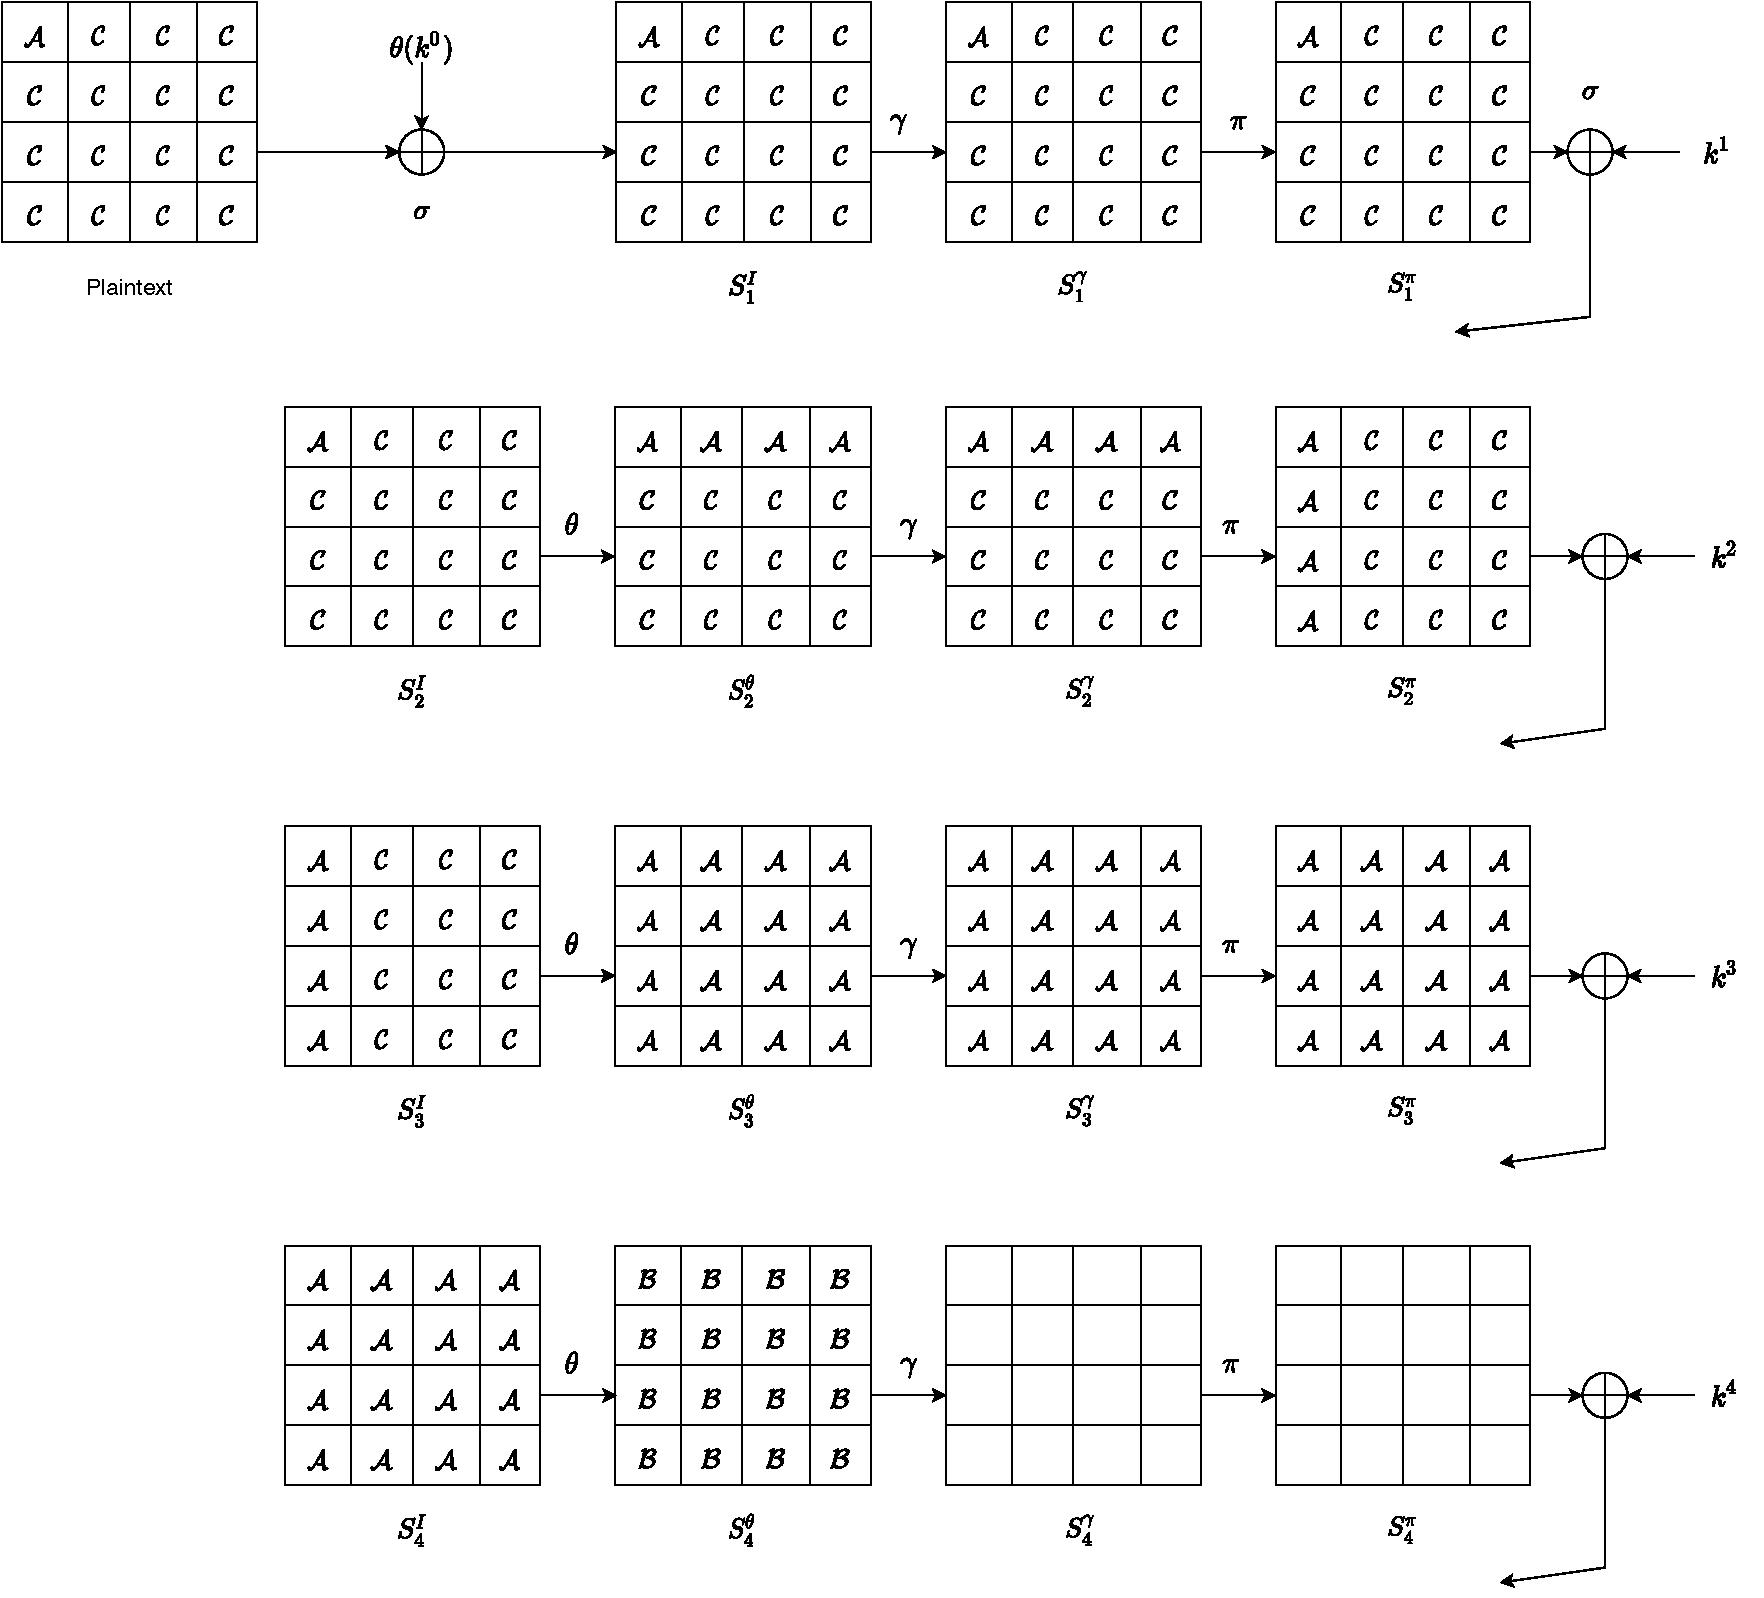
\includegraphics[width=\linewidth]{square_attack}
  \caption{Integral attack characteristic for 4 rounds}
  \label{fig:square_attack}
\end{figure}

\begin{flalign*}
  P_0 &= (0, c_1, c_2 \dotsc c_{15})\\
  P_1 &= (1, c_1, c_2 \dotsc c_{15})\\
  P_2 &= (2, c_1, c_2 \dotsc c_{15})\\
  &\vdots\\
  P_{255} &= (255, c_1, c_2 \dotsc c_{15})
\end{flalign*}

\begin{equation*}
  \Lambda = \{P_0, P_1, P_2 \dotsc P_{255}\}
\end{equation*}

The properties propagate through the rounds as shown in \autoref{fig:square_attack}. At the beginning of 4th round, all 16 positions have the All property. After the linear transformation $\theta$, all 16 positions have the balanced property as shown in \autoref{eq:bal}. A position is balanced if XOR sum of all 256 values is 0. It should be noted that All implies Balanced but the converse is not true.

\begin{flalign}
  \bigoplus_{0 \leq n \leq 255} S_{4,n}^\theta[i,j]
  &= \bigoplus_{0 \leq n \leq 255} \bigoplus_k c_{j-k} S_{4,n}^I[i,k] \label{eq:bal} \\
  &= \bigoplus_l c_l \bigoplus_{0 \leq n \leq 255} S_{4,n}^I[i,l+j] \nonumber \\
  &= \bigoplus_l c_l 0 \nonumber \\ &= 0 \nonumber
\end{flalign}

In the 4 round attack, we guess the value of a single byte $k_{i,j}^4$ of the round key $k^4$. Using $k_{i,j}^4$, we calculate the value of $S_4^\theta[j,i]$ for all 256 ciphertexts.

\begin{equation*}
  S_4^\theta[j,i] = Sbox^{-1}[S_5^I[i,j] \oplus k_{i,j}^4]
\end{equation*}

We verify whether the key guess was correct by calculating the XOR sum of all 256 values of $S_4^\theta[j,i]$. The key guess is discarded if the sum is non-zero. This is repeated for all bytes of the $k^4$. $k^4$ can be uniquely determined by using 2 $\Lambda$ sets of 256 plaintexts. Since the key schedule $\psi$ is invertible, the previous keys $k^0$ to $k^3$ can also be derived from $k^4$.

The attack can be extended from behind by guessing 4 bytes of $k^4$ and 4bytes of $k^5$ each time. 5 sets of 256 plaintexts are required for determining the key.

Another extension is possible from the beginning which involves crafting set of $2^32$ plaintexts such that the output of the first round has a column whose 4 byte value follows All property and the rest are Constant.

The complexity of different variations of the integral attack as in ~\cite{FSE:DaeKnuRij97} is shown in \autoref{tab:complexity}.

\begin{table}
  \centering
  \begin{tabular}{|c|c|c|c|}
    \hline
    Attack          & Plaintexts & Time  & Memory \\
    \hline
    4-round         & $2^9$      & $2^9$ & negl   \\
    5-round  type 1 & 211        & 240   & negl   \\
    5-round  type 2 & 232        & 240   & 232    \\
    6-round         & 232        & 272   & 232    \\
    \hline
  \end{tabular}

  \caption{Complexity of integral attack on SQUARE}
  \label{tab:complexity}
\end{table}


%%%% 8. BILBIOGRAPHY %%%%
\bibliographystyle{alpha}
\bibliography{cryptobib/abbrev3,cryptobib/crypto,biblio}
%%%% NOTES
% - Download abbrev3.bib and crypto.bib from https://cryptobib.di.ens.fr/
% - Use bilbio.bib for additional references not in the cryptobib database.
%   If possible, take them from DBLP.

\end{document}
